\begin{problem}{DOMINO}{DOMINO.inp}{DOMINO.out}{1s}{512M}
Bờm và Cuội gần đây đã tìm thấy một bảng trò chơi xếp hình domino cổ đại. Bảng có dạng hình chữ nhật được chia thành các lưới ô vuông kích thước $N\times M$, các hàng được đánh số từ $1$ đến $N$, các cột được đánh số từ 1 đến $M$, và $N$ và $M$ là các số tự nhiên lẻ. Bảng được lấp đầy bởi $\frac{N \times M - 1}{2}$ quân domino, mỗi domino chiếm hai ô liền kề, một số domino được đặt theo chiều ngang, một số lại được đặt theo chiều dọc, và rõ ràng sẽ có một ô trên bảng không bị quân domino nào đặt lên.

Bờm và Cuội nhìn vào bảng này và nghĩ về tất cả những nhiệm vụ tuyệt vời có thể nghĩ ra từ bảng xếp hình domino này. Một ý tưởng ngay lập tức nảy ra với họ. Với cách đặt các ô domino trên một bảng hiện tại, thì có thể di chuyển được bao nhiêu quân domino từ vị trí ban đầu của chúng đến vị trí khác, hay có bao nhiêu quân domino có thể thay đổi vị trí?

\centerline{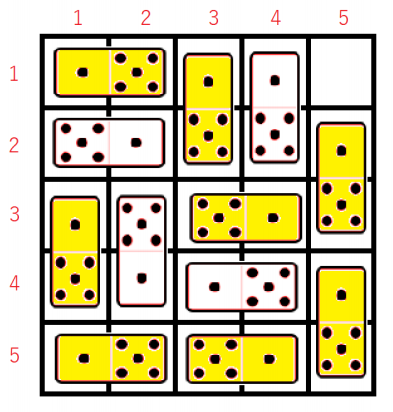
\includegraphics[totalheight=5cm]{domino/domino.PNG}}
    \label{fig:verticalcell}
    
Ví dụ, đối với một bảng được sắp xếp như trên, ô trống ở vị trí $(1,5)$, trước tiên chúng ta có thể di chuyển domino đặt trên các ô $(2,5), (3,5)$ lên trên và do đó, ô trống sẽ là ô $(3, 5)$. Sau khi di chuyển nó, nhiều khả năng hơn sẽ mở ra, vì vậy giả sử ta có thể di chuyển domino ở các ô $(4,5), (5,5)$ lên trên hoặc domino ở $(3,3), (3,4)$ về phía phải. 
Trong tổng số 12 quân cờ domino trên bảng này, tám quân trong đó có thể được di chuyển khỏi vị trí ban đầu của chúng theo một cách nào đó.

Hãy viết một chương trình đếm xem có bao nhiêu quân cờ domino khác nhau có thể được di chuyển ra vị trí khác theo một cách nào đó.

\InputFile
\begin{itemize}
    \item Dòng đầu tiên chứa hai số nguyên $N$ và $M$ là số hàng và số cột của bảng, cả hai đều là các số lẻ $(1 \le N, M < 500)$.
    \item Dòng thứ $i$ trong $\frac{N \times M - 1}{2}$ tiếp theo, mỗi dòng chứa bốn số nguyên dương $x_1, y_1, x_2, y_2$ tương ứng là vị trí đặt của quân domino thứ $i$ trên bảng là hai ô $(x_1, y_1)$ và $(x_2, y_2)$, với $x_1, x_2$ là chỉ số hàng và $y_1, y_2$ là chỉ số cột. Dữ liệu đảm bảo các quân domino không xếp chồng lên nhau, không vượt quá giới hạn của bảng, và hai ô của một quân domino đặt lên là hai ô kề nhau trên bảng. 
\end{itemize}
\OutputFile
\begin{itemize}
    \item Ghi ra một số nguyên duy nhất là số quân domino có thể di chuyển ra vị trí khác với vị trí ban đầu.
\end{itemize}

\Examples

\begin{example}%
\exmp{
5 5
4 3 4 4
4 5 5 5
5 2 5 1
1 2 1 1
3 4 3 3
5 4 5 3
4 1 3 1
3 2 4 2
2 3 1 3
2 5 3 5
1 4 2 4
2 1 2 2
}{
8
}%
\end{example}
\Scoring
\begin{itemize}
    \item Subtask 1: 45\% số điểm có $1 \le N, M \le 5$
    \item Subtask 2: 25\% số điểm có $N = M = 9$, và tối đa có 2 quân domino có thể di chuyển
    \item Subtask 3: 30\% số điểm còn lại không có ràng buộc gì thêm.
\end{itemize}
\end{problem}